%\externaldocument[-f]{c2_foundations}
%\externaldocument[-f]{c3_simulation_experiments}
\chapter{Results}
\label{chap:4}
The experimental results are presented in this chapter. First, the parameters for the variables introduced in \cref{chap:3} are given. Then a sample of simulated trajectories are shown as an example. Finally, the inference results are presented.

\section{Configurations}
\label{sec:config}
The configurations given below are used for the results presented in the following sections, if not specified otherwise.
\begin{itemize}
	\item Gamma priors for parent dynamics such that $ Q_{n} \sim \mathrm{Gam}(\symbf{\alpha}^n, \symbf{\beta}^n)$ for $n \in \left\lbrace 1,2\right\rbrace $, and $ \symbf{\alpha}^n = [\alpha^n_0, \alpha^n_1] $ and $ \symbf{\beta}^n = [\beta^n_0, \beta^n_1] $
	\begin{align}
	\symbf{\alpha}^1 = [5,10] &\quad \symbf{\beta}^1 = [5,20] \\
	\symbf{\alpha}^2 = [10,10] &\quad \symbf{\beta}^2 = [10,5]
	\label{eq:gamma_params}
	\end{align}
	\item Transition intensity matrices of $ X_1 $ and $ X_2 $ sampled from priors given above
	\begin{align}
	Q_1 &= 
	\begin{bmatrix}
	-1.117 & 1.117 \\
	0.836 &  -0.836
	\end{bmatrix} \\
	Q_2 &= 
	\begin{bmatrix}
	-1.1 & 1.1 \\
	2.445 &  -2.445
	\end{bmatrix}
	\end{align}
	\item Length of the trajectories $ T = 5\text{s} $
	\item State space $ \rchi_{P} = \rchi_1 \times \rchi_2 = \left\lbrace (x_1, x_2)\right\rbrace_{x_1\in \rchi_1, x_2\in \rchi_2} = \left\lbrace (0, 0), (0, 1), (1, 0),(1, 1)\right\rbrace $
	\item Observation space $ \mathcal{Y} = \left\lbrace 0, 1, 2 \right\rbrace $
	\item Action space $ \textit{A} = \left\lbrace a_{0}, a_{1} \right\rbrace = \left\lbrace 0, 1\right\rbrace $
	\item The set of transition intensity matrices of $ X_3 $
	\begin{align}
	\textbf{\textit{Q}}_3 = \left\lbrace Q_{3\mid a_{0}}, Q_{3\mid a_{1}} \right\rbrace = \left\lbrace 
	\begin{bmatrix}
	-0.5 & 0.5 \\
	2 &  -2
	\end{bmatrix}, 
	\begin{bmatrix}
	-3 & 3 \\
	0.02 &  -0.02
	\end{bmatrix} 
	\right\rbrace 
	\end{align}
	\item Number of particles $ M = 200 $
	\item Weights of the policy introduced in \autoref{eq:policy} $ \textbf{w} = [0.02, 0.833, 0.778, 0.87] $
	\item Observation model
	$\psi_{\text{true}} =
	\begin{bmatrix}
		1 & 0 & 0 \\
		0 & 1 & 0 \\
		0 & 1 & 0 \\
		0 & 0 & 1
	\end{bmatrix}$
%	\item Simulation parameters $  \theta_sim = \left\lbrace  \textbf{Q}_{1}, \textbf{Q}_{2}, \textit{\textbf{Q}}_3, \textbf{w}, \psi_{\text{true}} \right\rbrace $
\end{itemize}
%In the following, $ \psi_{\text{true}} $ denotes the observation model which is used for data generation in the given results.
\begin{figure}[t]
	\begin{center}
		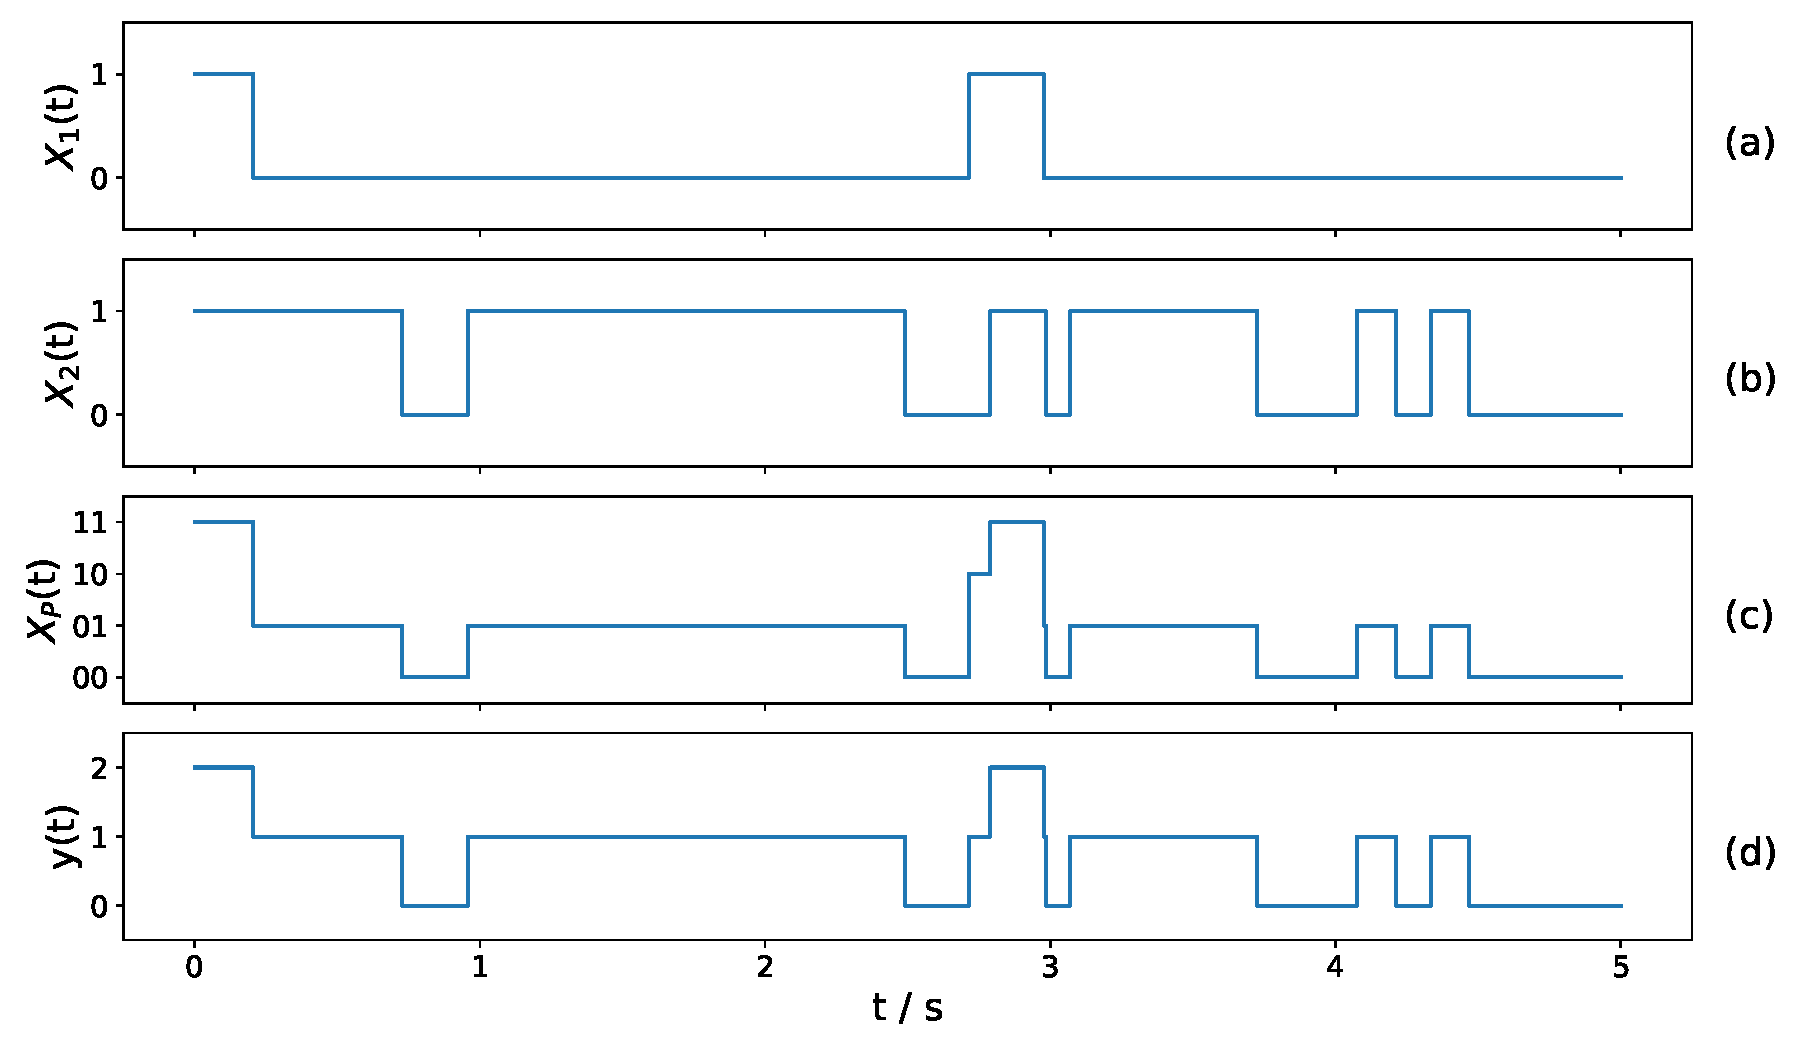
\includegraphics[width=.90\textwidth]{figures/sim_example/parent_traj}
		\caption[Parent trajectories and observation]{A sample of parent trajectories and observation. (a)-(b) A sample trajectory of parent nodes $ X_1 $ and $ X_2 $ of length $ T=5\text{s} $, (c) The trajectory of the joint parent process $ X_P $, (d) The observation trajectory resulting from $ X_P $ given in (c) and $ \psi_{\text{true}} $ given in \cref{sec:config}.}
		\label{fig:parent_traj}
	\end{center}
\end{figure}
\section{Simulation}
\label{sec:simulation}
The synthetic dataset is generated utilising \cref{alg:sampling}. $ K $ trajectories in time interval $ [0, T] $ are denoted by $ \xi_T = \left\lbrace S^{[0,T], 1}, S^{[0,T], 2}, ..., S^{[0,T], K} \right\rbrace  $, where $ S^{[0,T],\kappa} = \left\lbrace X_1^{[0,T],\kappa} , X_2^{[0,T],\kappa}, X_3^{[0,T],\kappa}\right\rbrace $ denotes a single trajectory for all nodes. It is noteworthy that the initial states are drawn from disrete uniform distribution.
\begin{equation}
X_n(0) \sim \mathcal{U} \left\lbrace 0, 1\right\rbrace  \text{ for } n \in \left\lbrace 1,2,3\right\rbrace 
\end{equation}
\autoref{fig:parent_traj}(a)-(b) shows an example of parent trajectories. In \autoref{fig:parent_traj}(c), the resulting trajectory of the joint parent process $ X_P $ is illustrated. As mentioned in \cref{sec:exp_ctbn_model}, this joint process over the parent nodes provides a compact representation. In \autoref{fig:parent_traj}(c), the states of $ X_P $ taking values in $ \rchi_P = \rchi_1 \times \rchi_2 $ is preferred to be represented as a combination of the parent states for readibility, so that $ \rchi_P = \left\lbrace 00, 01, 10, 11\right\rbrace  $, where $ x_P \in \rchi_P $ corresponds to $ x_1x_2,\ x_1\in \rchi_1,\  x_2\in \rchi_2 $. \autoref{fig:parent_traj}(d) shows the observation trajectory resulting from $ X_P(t) $ and the observation model $ \psi_{true} $ given in \cref{sec:config}. \\
\autoref{fig:belief_traj} illustrates the belief state trajectory given the observations in \autoref{fig:parent_traj}(d). For the reference, the belief state update using marginal particle filter and exact update are given together. Exact update of belief state is obtained as described in \cref{sec:exact_update}, while the marginal particle filter update is the result of sequential implementation of \cref{alg:part_filter}. For marginal particle filter, we plot the median as a line over 10 runs, and 25-75th percentile as the shaded area. As can be seen from the figures, the exact update is well approximated by the marginal particle filter.
\begin{figure}[t]
	\begin{center}
		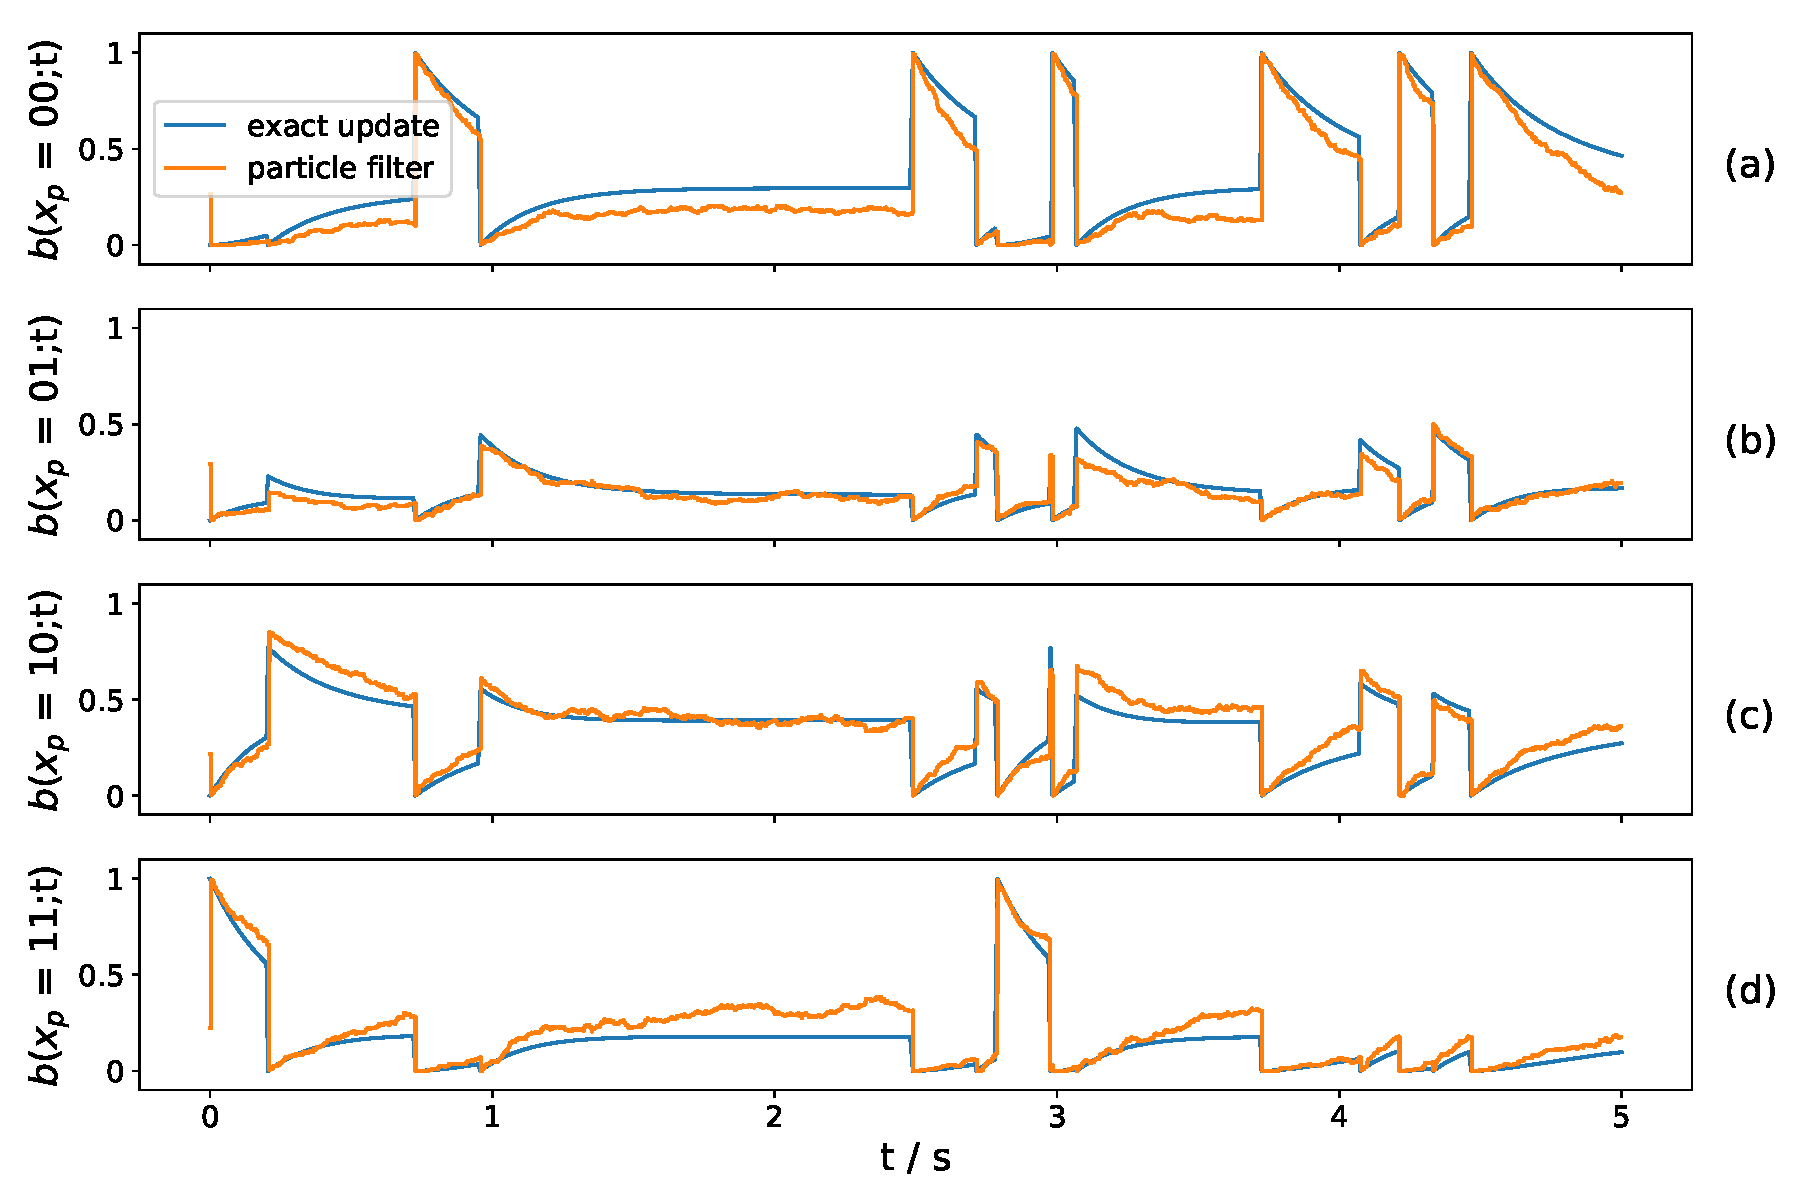
\includegraphics[width=.9\textwidth]{figures/sim_example/belief_traj}
		\caption[Belief state trajectories]{Belief state trajectories corresponding to the observations given in \autoref{fig:parent_traj}(d), comparing exact update method and marginal particle filtering.}
		\label{fig:belief_traj}
	\end{center}
\end{figure}\\
Finally, the resulting $ \textbf{Q}_3 $ and the trajectory of the agent are given in \autoref{fig:q_traj}. The $ Q_3 $ trajectory shown in \autoref{fig:q_traj}(b) is derived from the belief state update by marginal particle filter which is given in \autoref{fig:q_traj}(a) using \autoref{eq:policy} and \autoref{eq:Q_3_traj}.
\begin{figure}[t]
	\begin{center}
		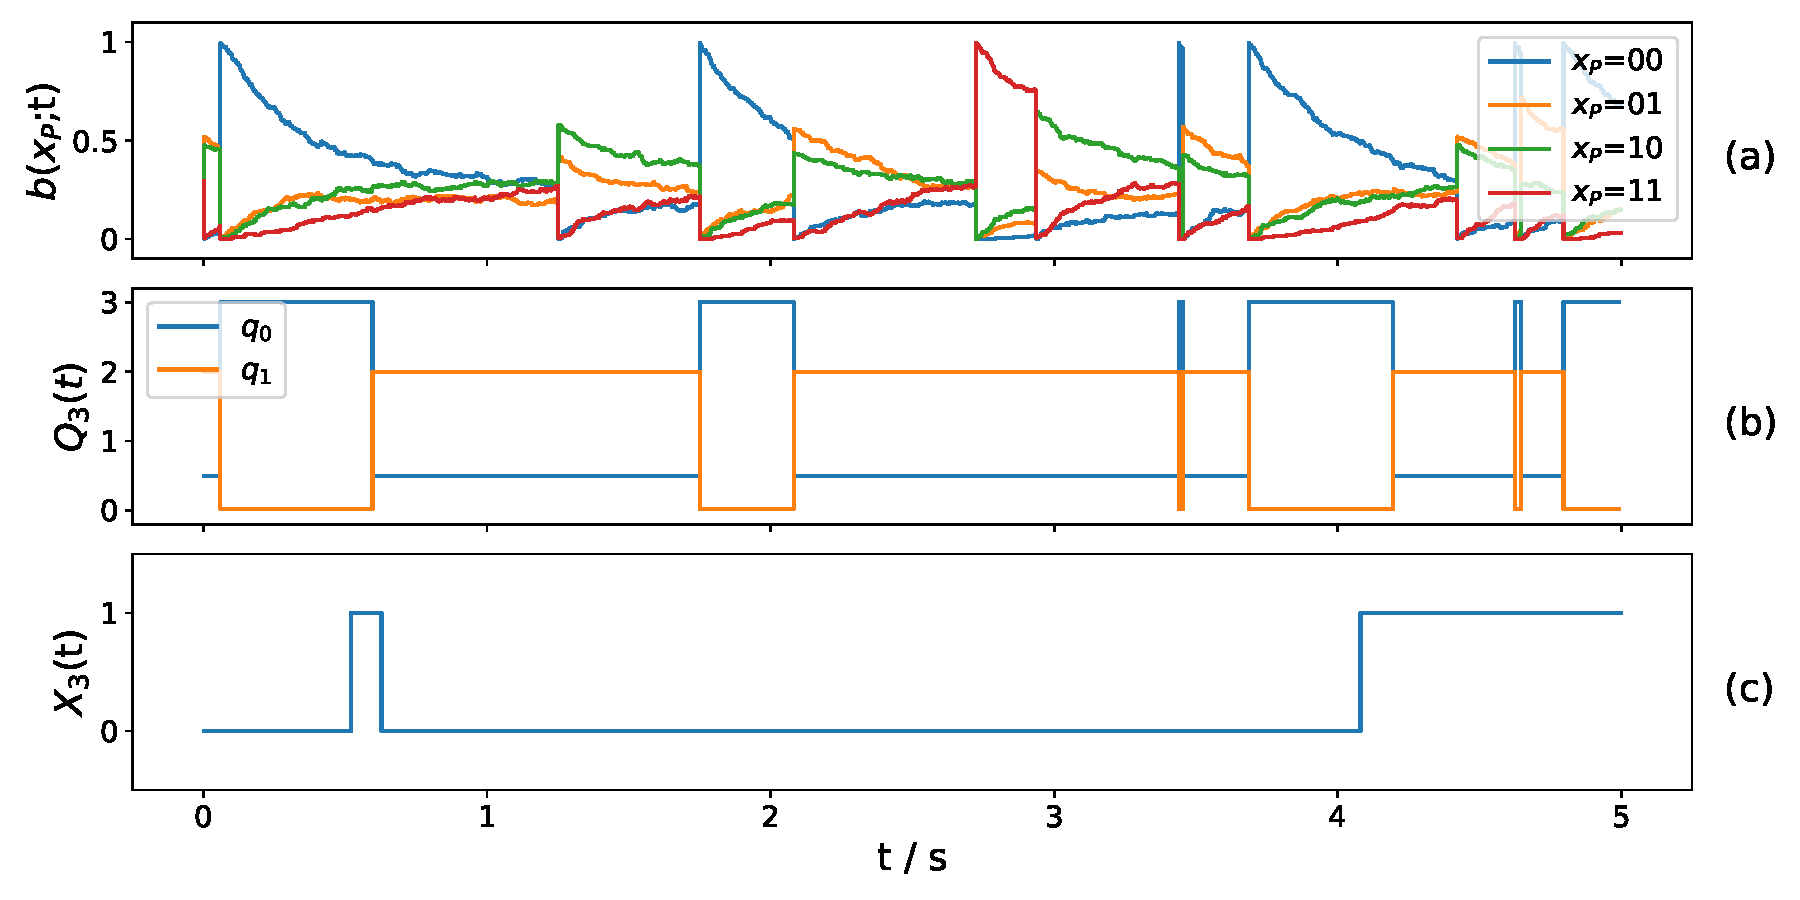
\includegraphics[width=.9\textwidth]{figures/sim_example/q_traj}
		\caption[$ Q_3 $ and $ X_3 $ trajectories]{Belief state updated by marginal particle filter and the resulting $ Q_3 $ and $ X_3 $ trajectories.}
		\label{fig:q_traj}
	\end{center}
\end{figure}\\
As mentioned in \cref{par:bs_partFilt}, the degeneration of the marginal particle filter in case of unlikely changes in observation, i.e. rapid transitions of parent nodes, is handled by assigning uniform weights to the particles. It effectively corresponds to ignoring these changes in the observation, which may cause divergence from the exact update. However, it is recovered with the next observation. \autoref{fig:deg_partFilter} provides an example of the situation. The rapid change in question is highlighted in \autoref{fig:deg_partFilter}(a). The particles fail to simulate this observation, and due to uniformization, the transition from 2 to 1 is ignored by the marginal particle filter method. The divergence can be observed in \autoref{fig:deg_partFilter}(d)-(e) clearly.
\begin{figure}[H]
	\begin{center}
		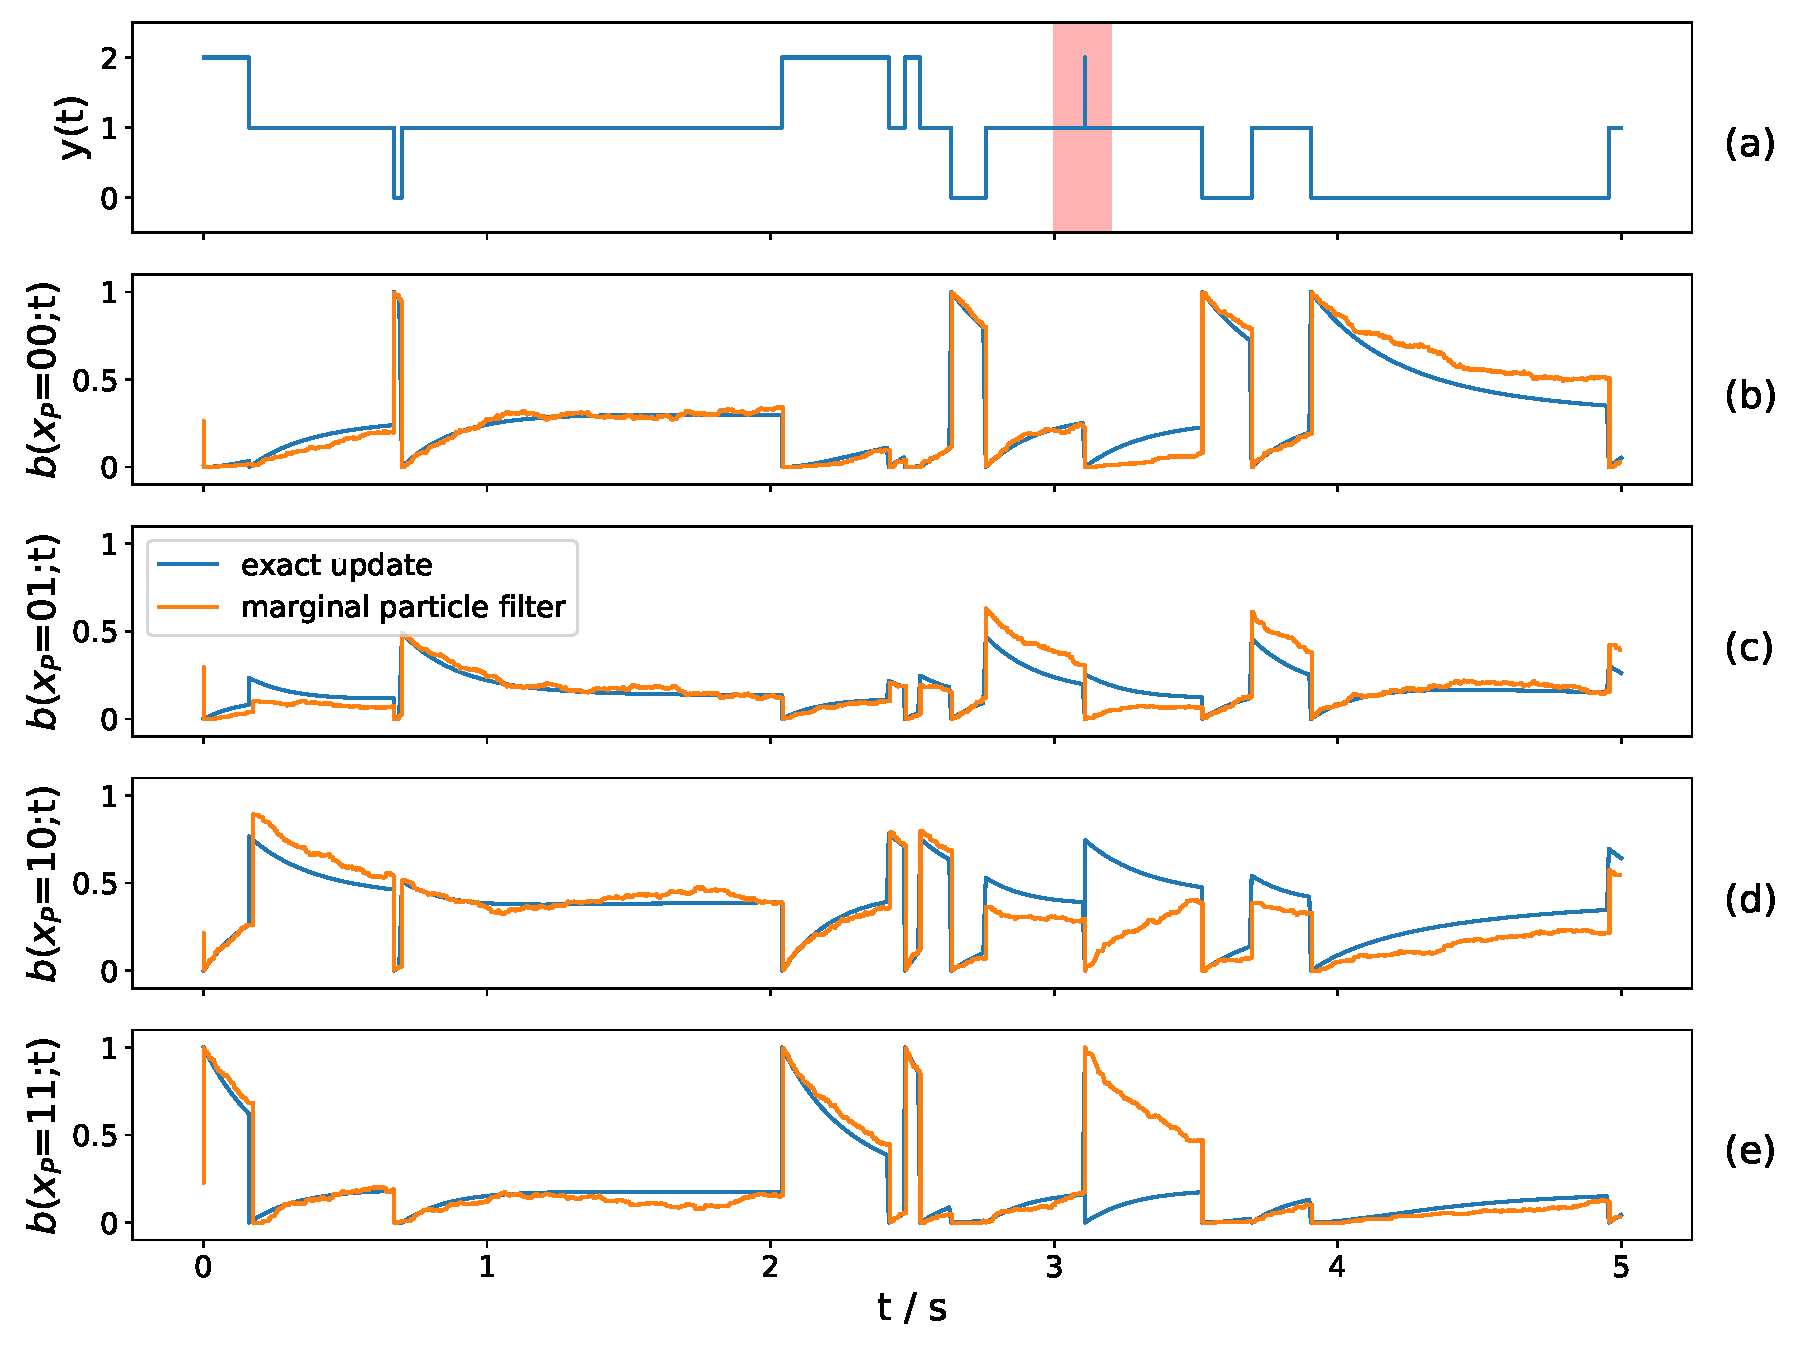
\includegraphics[width=.9\textwidth]{figures/degenerate_pf/belief_traj}
		\caption[Degenerate marginal particle filter]{A sample with degenerate marginal particle filter. The unlikely observation which has caused the degeneration is highlighted in (a). It can be seen in (d) and (e) that this observation causes particle filter approximation to diverge from exact update results but it is recovered with the next observation.}
		\label{fig:deg_partFilter}
	\end{center}
\end{figure}

\section{Inference of Observation Model}
In this section, the limitations to the classification problem are discussed and the results are presented.
\begin{figure}[t]
	\begin{center}
		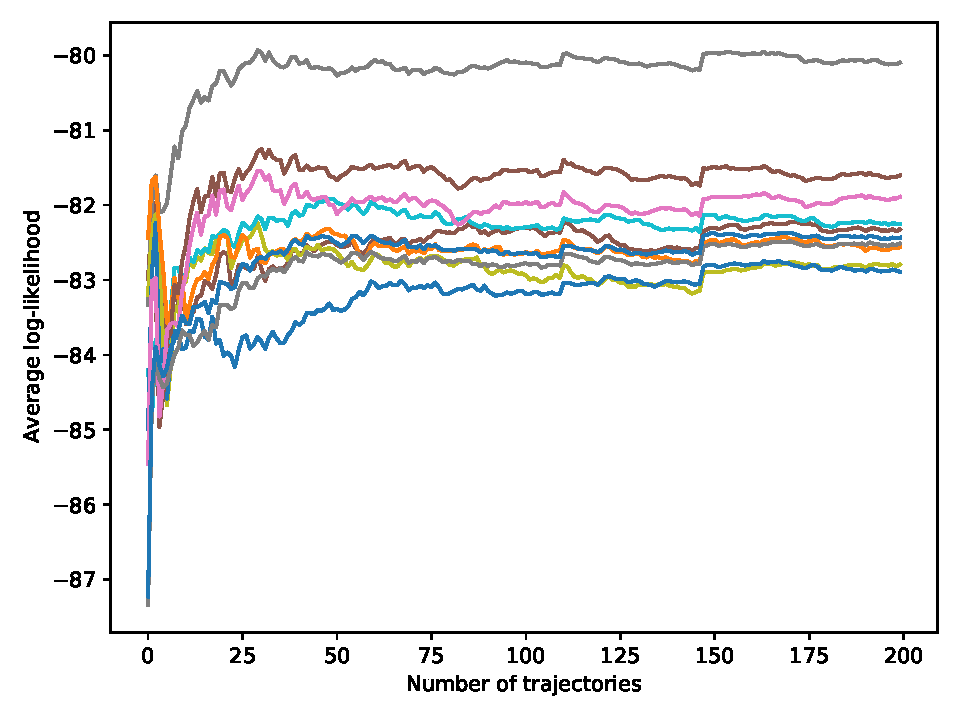
\includegraphics[width=.7\textwidth]{figures/equivalence_classes/llh_exactUpdate_81model}
		\caption[Equivalence classes in the case of exact belief update]{Average log-likelihood $ \log p(S^{[0,T]} \mid \theta) $ over samples generated using exact belief state update, depicting the equivalence classes in the set of observation models.}
		\label{fig:llh_exactUpdate_81model}
	\end{center}
\end{figure}
\subsection{Equivalence Classes}
\label{sec:eq_classes}
As mentioned in \cref{sec:inf_setup}, the deterministic nature of the observation model results in a number of possible observation models. The setting described in \cref{chap:3}, with configurations given in \cref{sec:config}, leads to 81 observation models. However, with this experimental setup and the methods, it is only possible to distinguish these observation models into 10 different classes. Due to this equivalence, the inference problem is considered only for 10 observation models, each one representing one class. The origins of this phenomena are discussed in detail in \cref{ap:eq_classes}, together with the observation models considered in the inference problem. The set of observation model that can be classified is denoted as $ \symbf{\psi} $ in the following. \\
\autoref{fig:llh_exactUpdate_81model} illustrates the equivalence of observation models clearly. The plot depicts the results of an experiment with 200 samples, $ |\xi_T| = 200 $, generated using the observation model $ \psi_{\text{true}} $ given in \cref{sec:config}, and the average log-likelihood of samples computed for all possible observation models. Here, the belief state is updated using exact method as described in \cref{par:bs_exact}, in order to depict the exact equivalence within one class. As can be seen, the results show the separation of the set of observation models into 10 distinct classes. The legend is removed to avoid clutter. The jump around 110 and 150 trajectories can be explained by an encounter with a sample of highly likely parent trajectories. Such encounters have the same affect on the likelihood of all observations, as can be seen from \autoref{eq:Marg_llh_final}.\\
In order to show the validity of the equivalence in the case of marginal particle filter, the average log-likelihoods of 200 samples given two observation models in the same class are illustrated in \autoref{fig:llh_particleFilter_sameclass}. The samples are generated with $ \psi_{\text{true}} = \psi_{0} $, and the rest of the observation models here fall in the same equivalence class as $ \psi_0 $. As can be seen from the graph, the observation models lead to such similar results that they are assumed to be identical. 
\begin{figure}[t]
	\begin{center}
		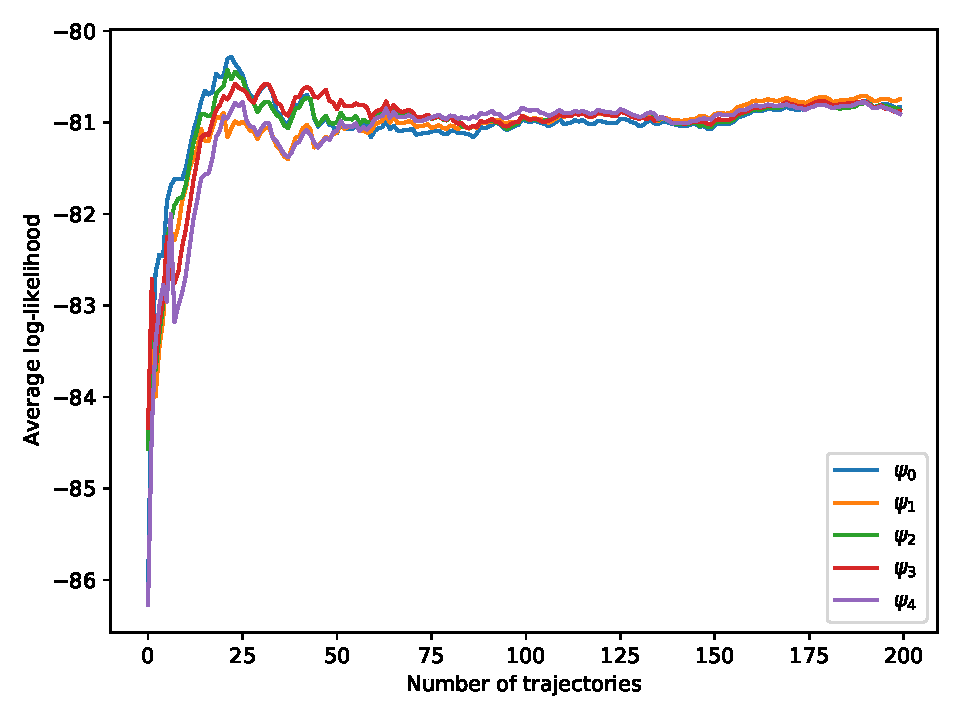
\includegraphics[width=.7\textwidth]{figures/equivalence_classes/llh_particleFilter_sameclass}
		\caption[An equivalence class in the case of marginal particle filtering]{Average log-likelihood $ \log p(S^{[0,T]} \mid \theta) $ over samples generated using marginal particle filtering, where $ \psi_1 $ and $ \psi_2 $ belongs in the same class.}
		\label{fig:llh_particleFilter_sameclass}
	\end{center}
\end{figure} 
\subsection{Learning Observation Model}
\autoref{fig:llh_exact} illustrates the average log-likelihood over 100 samples given the observation models. The samples are generated with $ \psi_{true} = \psi_0 $ given in \cref{sec:config}, and exact update method is utilised for belief state update. As can be seen, the curves converge quickly and the true model is well separated from others. Consequently, the maximum log-likelihood estimation, as given below, leads to the correct result. Here, in order to avoid numerical unstability, the log-likelihood is preferred for the calculations instead of likelihood.
\begin{equation}
\hat{\psi} = \argmax_\psi \left[ \log p(S^{[0,T]} \mid \theta )\right] 
\label{eq:max_llh_est}
\end{equation}
A similar experiment is documented in \autoref{fig:llh_particle}, where exact update method is replaced by marginal particle filtering. $ \psi_0 $ denotes the observation model that has generated the dataset, and it is correctly estimated as the true model. The jump around 50 trajectories can be explained by an encounter with a sample of highly likely parent trajectories.
\begin{figure}[H]
	\begin{center}
		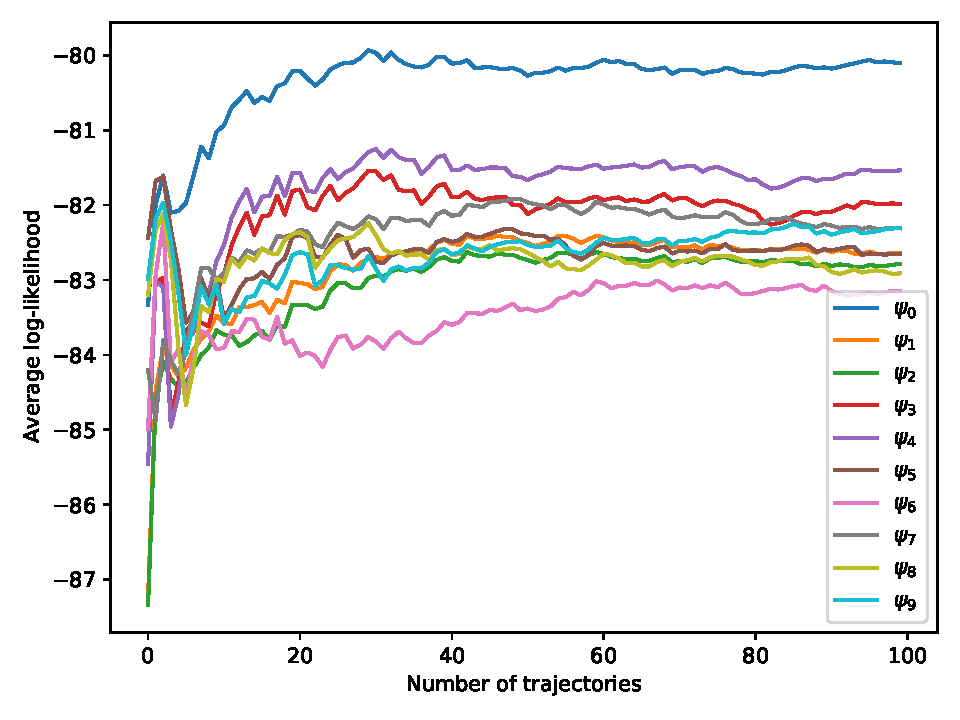
\includegraphics[width=.7\textwidth]{figures/roc_analysis/roc_exactUpdate/llh_exactUpdate_psi_0}
		\caption[Average log-likelihood in the case of exact belief update]{Average log-likelihood $ \log p(S^{[0,T]} \mid \theta) $ with $ \psi_i \in \symbf{\psi} $ over samples generated using exact belief state update}
		\label{fig:llh_exact}
	\end{center}
\end{figure}
\begin{figure}[H]
	\begin{center}
		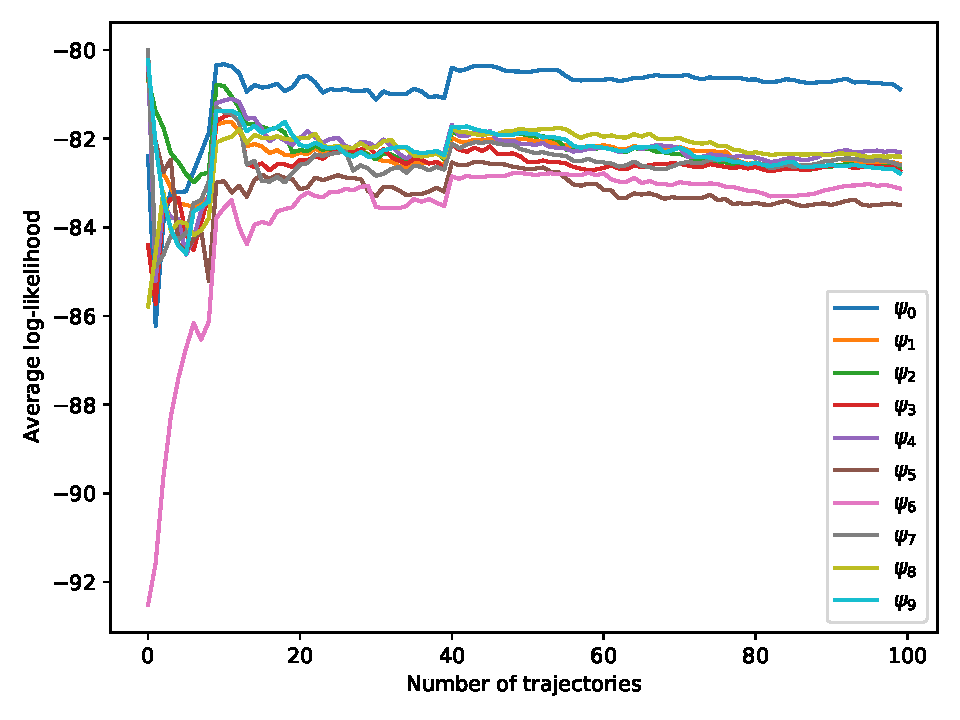
\includegraphics[width=.7\textwidth]{figures/roc_analysis/roc_particleFilter/llh_particleFilter_psi_0}
		\caption[Average log-likelihood in the case of marginal particle filtering]{Average log-likelihood $ \log p(S^{[0,T]} \mid \theta) $ with $ \psi_i \in \symbf{\psi} $ over samples generated using marginal particle filtering}
		\label{fig:llh_particle}
	\end{center}
\end{figure}
\pagebreak
We approach the inference problem as classification between the observation models $ \psi \in \symbf{\psi} $ given in \cref{ap:obs_set_exp}, and consider the estimated likelihood values of each sample given an observation model as the score of the sample belonging to the corresponding class. As a measure of the performance of the classifier, we utilise area under the Reciever-Operator-Characteristic curve (AUROC) and Precision-Recall curve (AUPR). Since this setting represents a multi-class classification problem, the performance metrics AUROC and AUPR are calculated as one-vs-rest. \\ %performance metric AUROC is calculated as one-vs-rest. \\ %
We have provided the classifier with increasing number of samples for inference. This is achieved through bootstrapping a given number of trajectories, and using the mean likelihood over the bootstrap batch as a new sample. The following AUROC plots shows the results over 50 trajectories generated using each obervation model as the true model. According to this, in our dataset, we have 500 trajectories, 50 from each class labeled through a vector with 10 entries, having a single element equal to 1 for the true observation model and 0 for the rest. When number of trajectories is 1, each sample in the dataset is considered individually. When number of trajectories is 2, within each class, 50 sample batches of size 2 are bootstrapped such that none of the batches consist of the same samples. By doing so, we keep the sample size at 50 per class, regardless of the batch size. \\
\autoref{fig:AUROC_class0} shows the AUROC results over 10 runs, comparing the state estimator using exact update and marginal particle filtering. We plot the median as a line and 25-75th percentile as the shaded area. The AUPR results are given in appendix \autoref{fig:AUPR_class0} in the same manner. As expected given the unbiased classifier, both metrics approach to 1 as the number of samples increases. Due to the stochasticity introduced by the marginal particle filtering as the state estimator, the results obtained with this method show slightly lower performance. 
%As expected given the unbiased classifier, this metric approaches to 1 as the number of samples increases. Due to the stochasticity introduced by the particle filtering as the state estimator, the results obtained with this method show slightly lower performance. 
%\begin{figure}[t]
%	\begin{subfigure}{.5\textwidth}
%		\begin{center}
%			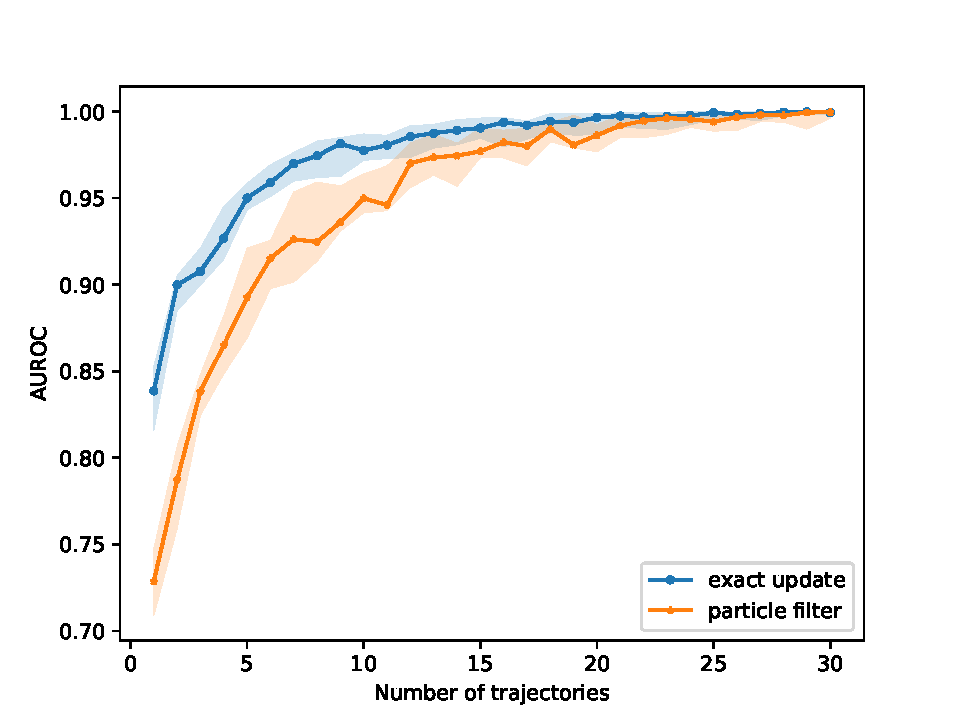
\includegraphics[width=1\textwidth]{figures/roc_analysis/AUROC_perc_0}
%%			\caption[AUROC results over increasing number of samples]{AUROC results over increasing number of samples for $ \psi_0 $-vs-rest. We plotted the median with line and the 25-75\% percentile with the shaded area over 10 runs.}
%			\label{fig:AUROC_class0}
%		\end{center}
%	\end{subfigure}
%	\begin{subfigure}{.5\textwidth}
%		\begin{center}
%			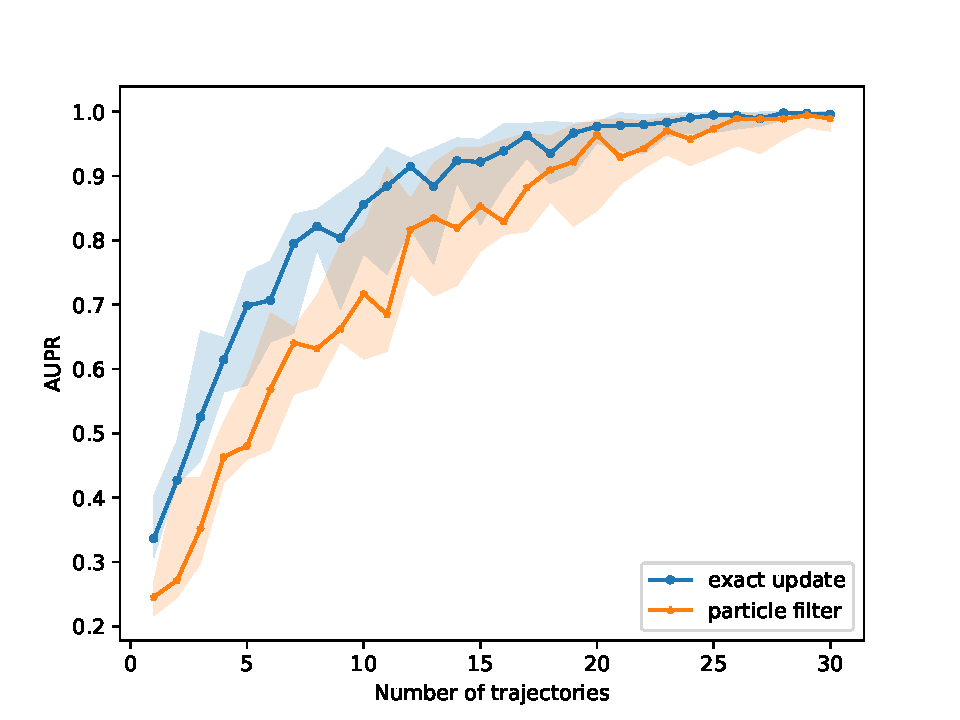
\includegraphics[width=1\textwidth]{figures/roc_analysis/AUPR_perc_0}
%%			\caption[AUPR results over increasing number of samples]{AUPR results over increasing number of samples for $ \psi_0 $-vs-rest. We plotted the median with line and the 25-75th percentile with the shaded area over 10 runs.}
%			\label{fig:AUPR_class0}
%		\end{center}
%	\end{subfigure}
%	\caption[AUPR results over increasing number of samples]{AUPR results over increasing number of samples for $ \psi_0 $-vs-rest. We plotted the median with line and the 25-75th percentile with the shaded area over 10 runs.}
%\end{figure}
\begin{figure}[t]
	\begin{center}
		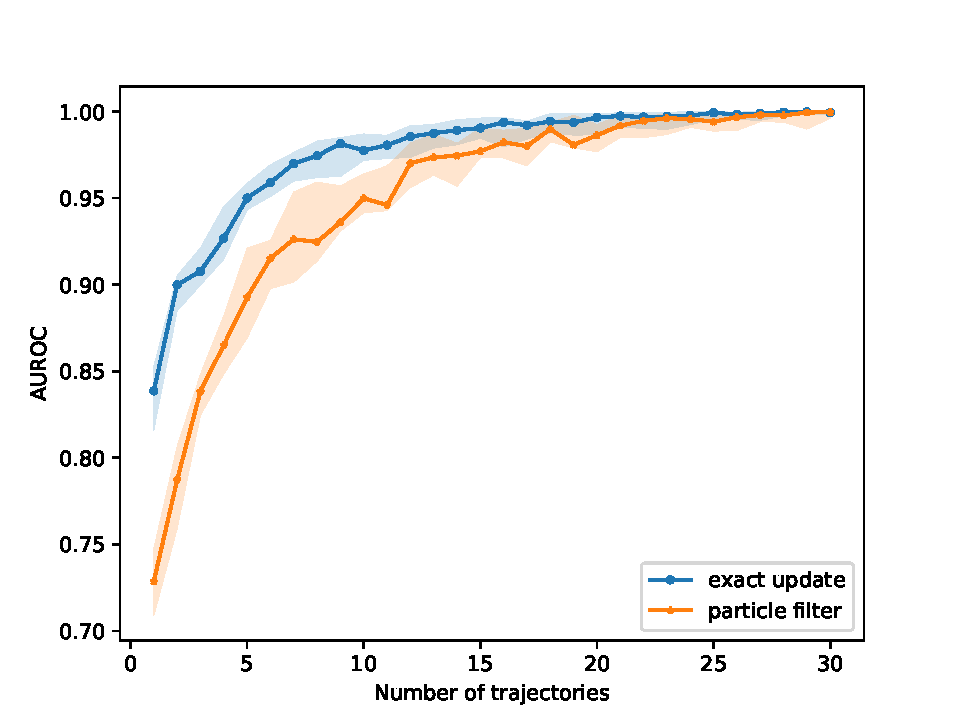
\includegraphics[width=0.75\textwidth]{figures/roc_analysis/AUROC_perc_0}
		\caption[AUROC results over increasing number of samples]{AUROC results over increasing number of samples for $ \psi_0 $-vs-rest. We plot the median with a line and the 25-75\% percentile with the shaded area over 10 runs.}
		\label{fig:AUROC_class0}
	\end{center}
\end{figure}

\begin{figure}[t]
	\begin{center}
		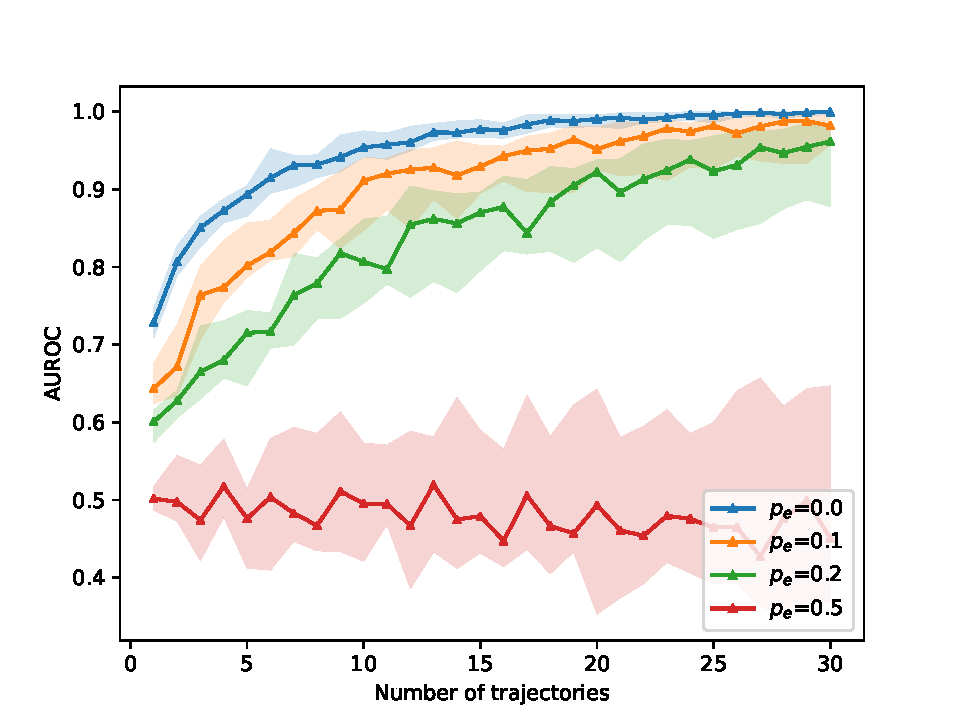
\includegraphics[width=.75\textwidth]{figures/roc_analysis/error_AUROC_perc_0}
		\caption[AUROC results over increasing number of samples with different error probability $ p_e $]{AUROC results over increasing number of samples for $ \psi_0 $-vs-rest. We plot the median with a line and the 25-75\% percentile with the shaded area over 10 runs. The performance deteriorates as the noise increases, however, with the increasing number of trajectories the metric converges to 1, showing the robustness.}
		\label{fig:AUROC_class0_error}
	\end{center}
\end{figure}
\subsection{Inference under Noisy Observation Model}
We have experimented with some added noise to the observation model, to test the robustness of the inference. How this noise was introduced to the observation model and how it affects the resulting observation is discussed in \cref{sec:noisy_robustness}. The noise is quantified with an error probability $ p_e $ of the observation model leading to a wrong observation. The noisy observation model can be interpreted as a noisy communication channel with error probability $ p_e $. \\
AUROC results for different levels of noise are given in \autoref{fig:AUROC_class0_error}. We plot the median as a line and 25-75th percentiles are shown as the shaded area around. The performance decreases as the noise introduced to the true observation model increases. These results confirm the expectations, as the noise leads to less reliable observations for the agent. On the other hand, with the increasing number of trajectories the metric converges to 1, showing robustness. The error probability of 0.5 shows the break point, at which the classes are no longer separable for the classifier. 
\pagebreak

\begin{figure}[H]
	\begin{subfigure}{.5\textwidth}
		\centering
		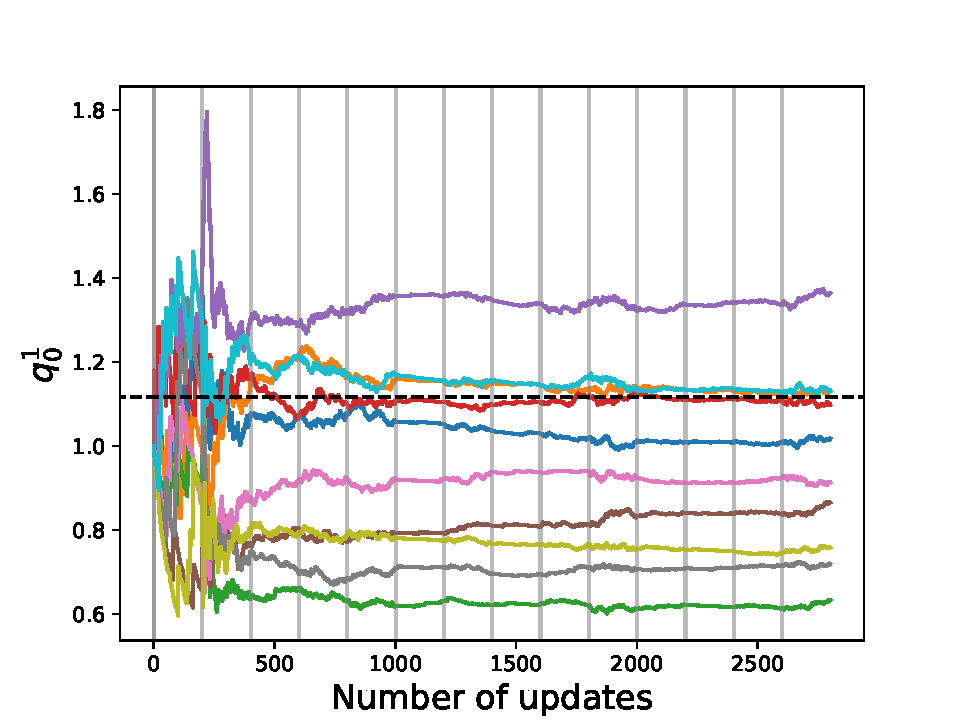
\includegraphics[width=1\linewidth]{figures/q_convergence/Q1_01}
		\caption{}
		\label{fig:Q1_01}
	\end{subfigure}
	\begin{subfigure}{.5\textwidth}
		\centering
		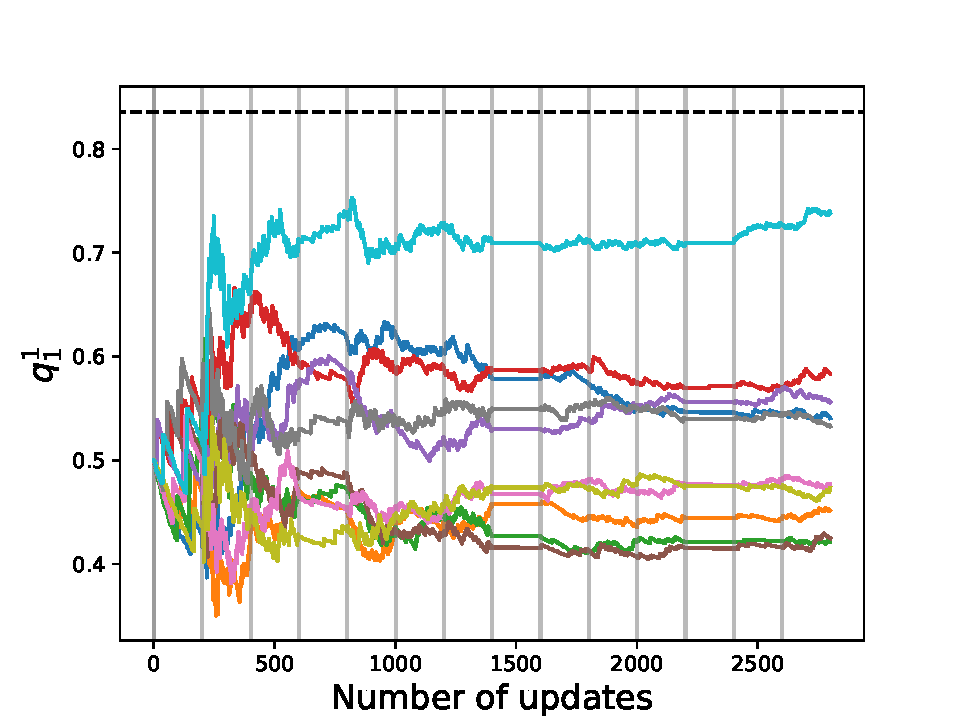
\includegraphics[width=1\linewidth]{figures/q_convergence/Q1_10}
		\caption{}
		\label{fig:Q1_10}
	\end{subfigure}\\
	\begin{subfigure}{.5\textwidth}
		\centering
		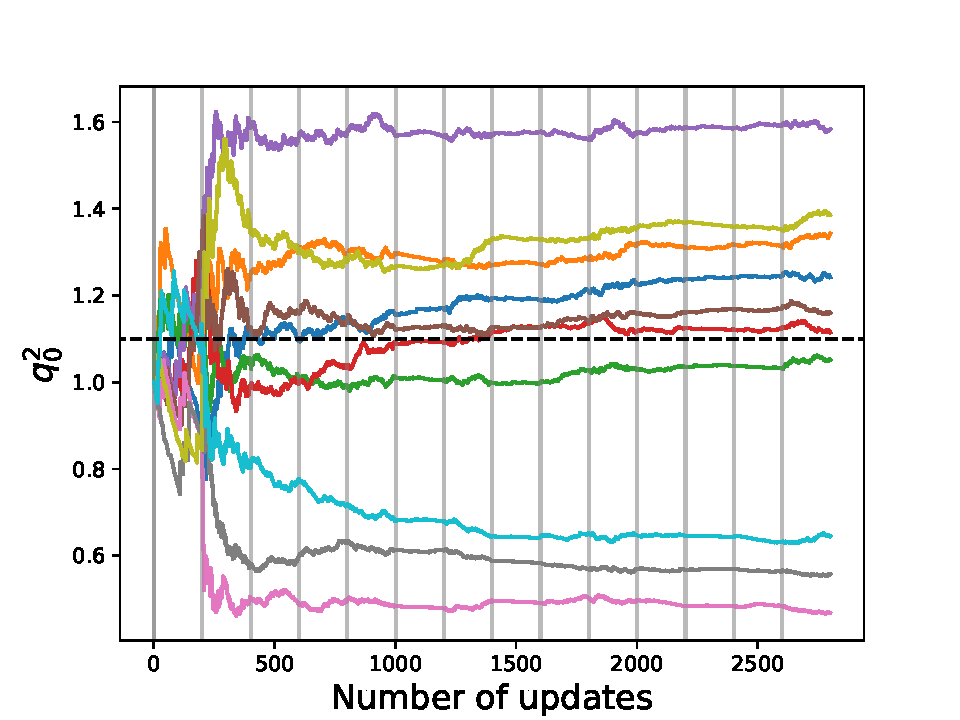
\includegraphics[width=1\linewidth]{figures/q_convergence/Q2_01}
		\caption{}
		\label{fig:Q2_01}
	\end{subfigure}
	\begin{subfigure}{.5\textwidth}
		\centering
		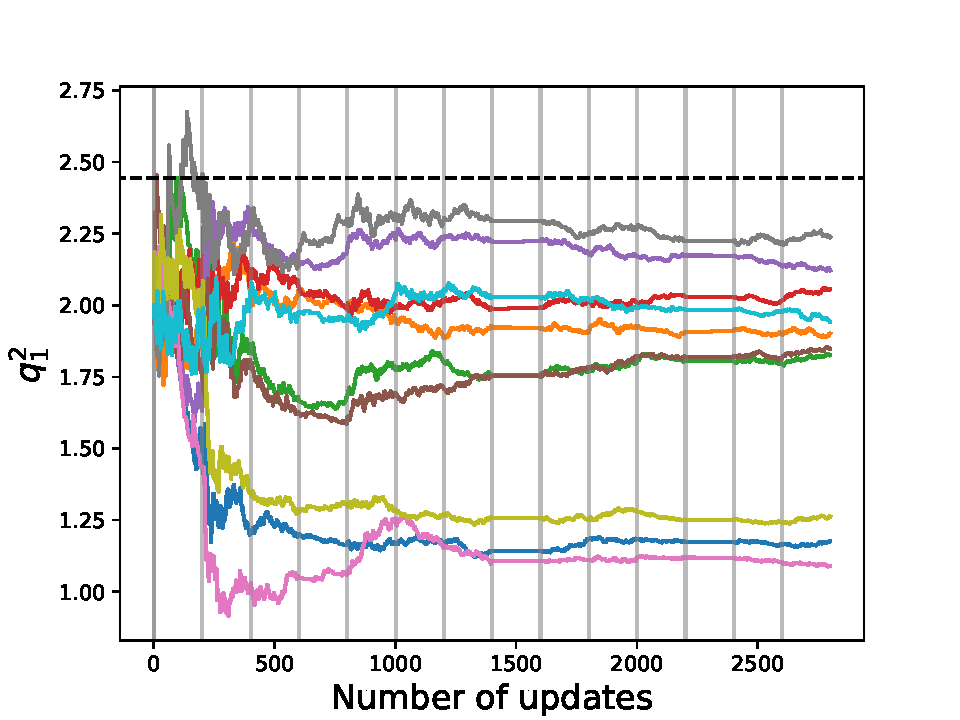
\includegraphics[width=1\linewidth]{figures/q_convergence/Q2_10}
		\caption{}
		\label{fig:Q2_10}
	\end{subfigure}
	\caption[Estimation of $ Q_1 $ and $ Q_2 $ by marginal particle filter]{Estimated transition intensities of $ Q_1 $ and $ Q_2 $ by marginal particle filter. Each colored line illustrates one estimation from 10 particle filters shown in \autoref{fig:belief_traj}. The notation on y-axis label follows the notation in \autoref{eq:Q_parents}. Black dashed line marks the true values of the transition intensity. The gray lines show the observations. Between each observation, there are 200 updates to the estimation, each coming from one particle.}
	\label{fig:q_convergence}
\end{figure}
\subsection{Estimated Intensity Matrices by Marginal Particle Filter}
In marginal particle filtering, the belief state is formed over particles drawn from marginalized processes of parents as in \autoref{eq:belief_over_particles}. In order to achieve this, the intensity matrices are replaced with the expectation given in \autoref{eq:estimated_Q}. With every new observation, the particles are propagated through the marginal process and the summary statistics are updated after each particle. Gamma-priors of the parent transition intensities are given in \cref{sec:config}. \\
In \cref{sec:simulation}, we have presented an example of sampled trajectories. \autoref{fig:parent_traj} illustrates the parent trajectories, and \autoref{fig:belief_traj} shows the belief state updated using exact method, and marginal particle filtering. For the latter, we plotted the statistics over 10 filters. \autoref{fig:q_convergence} illustrates the estimated transition intensities of those 10 particle filters. The notation on y-axis label follows the notation in \autoref{eq:Q_parents}. Each colored line illustrates one estimation from 10 particle filters shown in \autoref{fig:belief_traj}. Black dashed line marks the true values of the transition intensity. The gray lines show the observations. Between each observation, there are 200 updates to the estimation, each coming from one particle. \\
As can be seen from the figures, the estimations converge, although the final estimated value might be different than the true values. This can be explained by the fact that at the early stages, an unlikely transition sampled from marginal process causes a significant change in the estimation, which in return affects the distribution from which the next transitions are drawn. Such significant ripples can be seen at the early updates, i.e. updates 0 to 500 in the course of first 3 observations, which play a major role on the value the estimation converges to.
%\begin{align}
%\textbf{Q}_i = 
%\begin{bmatrix}
%-q^i_{0} & q^i_{0} \\
%q^i_{1} &  -q^i_{1}
%\end{bmatrix}
%\label{eq:Q_parents}
%\end{align}
